\documentclass{article}

\usepackage[margin=1.6in]{geometry}

\title{The fundamental group of the projective line minus three points}
\author{P. Deligne}
\date{1989}

\newcommand{\doctype}{French paper}
\newcommand{\origcit}{%
  \textsc{Deligne, P.}
  "Le Groupe Fondamental de la Droite Projective Moins Trois Points."
  In \emph{Galois Groups over $\mathbb{Q}$}, Springer-Verlag, Mathematical Sciences Research Institute Publications, Volume~\textbf{16} (1989), 79--297.
  DOI: \href{https://doi.org/10.1007/978-1-4613-9649-9_3}{\texttt{10.1007/978-1-4613-9649-9\_3}}%
}


\usepackage{amssymb,amsmath}

\usepackage{hyperref}
\usepackage{xcolor}
\hypersetup{colorlinks,linkcolor={blue!50!black},citecolor={blue!50!black},urlcolor={blue!80!black}}
\usepackage{enumerate}
\usepackage{tikz}
\usepackage{tikz-cd}
\usepackage{mathtools}

\usepackage{mathrsfs}
%% Fancy fonts --- feel free to remove! %%
\usepackage{fouriernc}


\usepackage{fancyhdr}
\usepackage{lastpage}
\usepackage{xstring}
\pagestyle{fancy}
\fancypagestyle{plain}{}
\fancyhf{}
\lhead{\footnotesize\nouppercase\leftmark}
\cfoot{\small\thepage\ of \pageref*{LastPage}}
% Git commit hash for server builds
\newif\ifserver
\serverfalse
\lfoot{\footnotesize\ifserver{Git commit: \href{https://github.com/thosgood/translations/commit/GitCommitHashVariable}{GitCommitHashVariable}}\fi}



\setcounter{section}{-1}
\usepackage{titlesec}
\titleformat{\section}[block]
  {\bfseries\Large\filcenter}
  {\S\thesection.}
  {1em}
  {}


%% Theorem environments %%

\usepackage{amsthm}

\theoremstyle{definition}

\newtheorem{innerenv}{}
\newenvironment{env}[1]
  {\renewcommand\theinnerenv{(#1)}\innerenv}
  {\endinnerenv}


%% Shortcuts %%

\newcommand{\mot}{\mathrm{mot}}
\newcommand{\scr}[1]{{\mathscr{#1}}}
\renewcommand{\cal}[1]{{\mathcal{#1}}}
\newcommand{\bb}{\mathbb}
\newcommand{\PP}{\bb{P}}
\newcommand{\ZZ}{\bb{Z}}
\newcommand{\hZZ}{\widehat{\bb{Z}}}
\newcommand{\RR}{\bb{R}}
\renewcommand{\AA}{\bb{A}}
\newcommand{\CC}{\bb{C}}
\newcommand{\FF}{\bb{F}}
\newcommand{\QQ}{\bb{Q}}
\newcommand{\cQQ}{\overline{\QQ}}
\newcommand{\DR}{{\mathrm{DR}}}

\renewcommand{\geq}{\geqslant}
\renewcommand{\leq}{\leqslant}

\DeclareMathOperator{\Gal}{Gal}
\DeclareMathOperator{\Lie}{Lie}
\DeclareMathOperator{\Ext}{Ext}
\DeclareMathOperator{\Spec}{Spec}
\DeclareMathOperator{\Hom}{Hom}
\DeclareMathOperator{\limind}{lim\,ind}
\DeclareMathOperator{\limproj}{lim\,proj}
\DeclareMathOperator{\HH}{H}

\DeclareMathOperator{\shIsom}{\underline{Isom}}

\newcommand{\unsure}[1]{TODO: \underline{\textbf{#1}}}
\newcommand{\todo}{\textbf{ !TODO! }}
\newcommand{\oldpage}[1]{\marginpar{\footnotesize$\Big\vert$ \textit{p.~#1}}}


%% Document %%

\usepackage{embedall}
\begin{document}

\maketitle
\thispagestyle{fancy}

\renewcommand{\abstractname}{Translator's note.}

\begin{abstract}
  \renewcommand*{\thefootnote}{\fnsymbol{footnote}}
  \emph{This text is one of a series\footnote{\url{https://thosgood.com/translations}} of translations of various papers into English.}
  \emph{The translator takes full responsibility for any errors introduced in the passage from one language to another, and claims no rights to any of the mathematical content herein.}

  \medskip
  
  \emph{What follows is a translation of the \doctype:}

  \medskip\noindent
  \origcit
\end{abstract}

\setcounter{footnote}{0}

\tableofcontents
\bigskip


%% Content %%


\section*{Leitfaden}
\[
  \begin{tikzcd}[row sep=1em]
    1 \ar[dd, no head] & 4 \ar[d, no head] & & 9 \ar[d, no head] &
  \\& 5 \ar[d, no head] & & 10 \ar[dl, no head] \ar[dr, no head] &
  \\2 \ar[dd, no head] \ar[dr, no head] & 6 \ar[d, no head] & 11 \ar[ddr, no head] & & 12 \ar[ddl, no head]
  \\& 7 \ar[d, no head] \ar[drr, no head] & & &
  \\3 \ar[dddddrr, no head] & 8 & & 13 \ar[d, no head] &
  \\ & & & 14 \ar[d, no head] &
  \\ & & & 15 \ar[d, no head] &
  \\ & & & 16 \ar[d, no head] \ar[dr, no head] \ar[ddl, no head] &
  \\ & & & 17 \ar[dl, no head, dashed] & 18
  \\ & & 19 & &
  \end{tikzcd}
\]


\section*{}

\oldpage{3~(81)}
The present article owes much to A.~Grothendieck.
He invented the philosophy of motives, which is our guiding thread.
Around five years ago, he also said to me, with conviction, that the profinite completion $\hat{\pi}_1$ of the fundamental group of $X\coloneqq\PP^1(\CC)\setminus\{0,1,\infty\}$, with the action of $\Gal(\cQQ/\QQ)$, is a remarkable object, and that it must be studied.

Every finite cover of $X$ can be described by equations with coefficients in the algebraic numbers.
Applying an element of $\Gal(\cQQ/\QQ)$ to these coefficients, we obtain the equations of another cover.
Understanding how $\Gal(\cQQ/\QQ)$ permutes the isomorphism classes of finite covers essentially reduces to understanding the Galois action on $\hat{\pi}_1$.
``Essentially'', since I have omitted mentioning the base points, and since the Galois covers have not been thought of as $G$-covers, for $G$ their automorphism group.

Up until now, we have not had the language necessary to study the Galois action on $\hat{\pi}_1$.
A.~Grothendieck and his students have developed a combinatorial description (``charts'') of finite covers of $X$, based on a decomposition of $\PP^1(\CC)$ into the two ``spherical triangles'' $\Im(z)\geq0$ and $\Im(z)\leq0$, with sides $[\infty,0]$, $[0,1]$, and $[1,\infty]$.
This has not helped in understanding the Galois action.
We have only a few unresolved examples of covers whose Galois conjugates have been calculated.

In this article, we only consider when $\hat{\pi}_1$ is rendered nilpotent, i.e. quotients $\hat{\pi}_1^{(N)}$ of $\hat{\pi}_1$ by the subgroups of its decreasing central series.
The profinite group $\hat{\pi}_1^{(N)}$ is a product over primes $\ell$ of nilpotent pro-$\ell$-groups: $\hat{\pi}_1^{(N)} = \prod_\ell \hat{\pi}_1^{(N)}{}\!_\ell$.
Each $\hat{\pi}_1^{(N)}{}\!_\ell$ is an $\ell$-adic Lie group.
It admits a Lie algebra $\Lie\hat{\pi}_1^{(N)}{}\!_\ell$, which is a Lie algebra over $\QQ_\ell$.
If we choose a base point $x\in X(\QQ)=\QQ\setminus\{0,1\}$, then $\Gal(\cQQ/\QQ)$ acts on these Lie algebras.
The action, up to inner automorphism, does not depend on the choice of $x$.
We would like to understand these actions.

The nilpotent versions of $\pi_1$ is very close to cohomology.
This is most visible in the theory of D.~Sullivan (\cite{Su}, \cite{Mo}).
Notation: for $\Gamma$ a finitely generated group, let $Z^i\Gamma$ be the decreasing central series, let $\Gamma^{(N)}=\Gamma/Z^{N+1}\Gamma$, and let $\Gamma^{[N]}=\Gamma^{(N)}/\mathrm{torsion}$ \hyperref[9.3]{(9.3)}.
The theory of Malcev (\cite{Mal}) attaches a nilpotent Lie algebra over $\QQ$, denoted $\Lie\Gamma^{[N]}$, to $\Gamma^{[N]}$, such that $\Gamma^{[N]}$ is a congruence subgroup of the unipotent algebraic group over $\QQ$ of the Lie algebra $\Lie\Gamma^{[N]}$.
By D.~Sullivan, if $X$ is a differentiable manifold, then $\Lie\pi_1(X)^{[N]}\otimes\RR$ is determined, up to inner automorphism, by the differential-graded algebra $\Omega_X^\bullet$, taken
\oldpage{4~(82)}
up to quasi-isomorphism.

This close relation with cohomology hints that the study of nilpotent versions of $\hat{\pi}_1$ is far from the ``anabelian'' dream of A.~Grothendieck.
It allows us, however, to use his philosophy of motives.

Let $k$ be a number field.
If $X$ is an algebraic variety over $k$, then we have a whole series of parallel cohomology theories for $X$: the classical cohomology of $X(\CC)$ (for each complex embedding of $k$), crystalline cohomology (which is equal to de Rham cohomology if $X$ is smooth), $\ell$-adic cohomology, \ldots.
The groups thus obtained are endowed with various additional structures (Hodge mixed, Galois action, \ldots) and are linked by comparison isomorphism.
In \hyperref[1]{\S1}, we axiomatise the situation by defining ``realisation systems over $k$''.
The exact definition is not to be taken seriously: considering the applications --- and what we are capable of doing --- it could be wise to either add or remove data as much as axioms.
The essential, for us, is that
\begin{enumerate}[(i)]
  \item The category of realisation systems is endowed with a $\otimes$ satisfying the usual properties: it is a Tannakian category over $\QQ$.
  \item Conjecturally, the category of motives is a full subcategory of the category of realisation systems.
\end{enumerate}

Condition~(ii) requires, in particular, that, for every variety $X$ over $k$ and for every $i$, the available cohomology theories, applied to $X$, give a realisation system $H^i(X)$ over $k$ (which we will denote by $H^i(X)_\mot$, and call the motivic $H^i$ of $X$).

Analogous ideas have been independently developed by U.~Jannsen \cite{J}.
In \cite{J}, U.~Jannsen defines (mixed) motives over $k$ as constituting the Tannakian subcategory (of the category of realisation systems) generated by the $H^i(X)$ for $X$ smooth and quasi-projective.
Here we are still being imprecise, saying that a motive over $k$ is a realisation system ``of geometric origin''.
For $X$ over $k$ and $x\in X(k)$, we want, for example, to regard $\Lie\pi_1(X(\CC),x)^{[N]}$ as a realisation of a motive over $k$.

This article owes much to an unpublished work of Z.~Wojtkoviak.
For $X=\PP^1\setminus\{0,1,\infty\}$ and $x\in X(\CC)$, I proposed to him a definition of the mixed Hodge structure of $\Lie\pi_1(X(\CC),x)^{[N]}$.
He calculated it in part, for small $N$, and, to my extreme surprise, show that, for $N=4$, its description involves $\zeta(3)$.
A decanted form of the calculations appear in \hyperref[19]{\S19}.
In fact, the whole article originates from my desire to
\oldpage{5~(83)}
understand the result of Z.~Wojtkoviak.
I have also been helped by the answer by O.~Gabber to my question ``How can we construct an extension of $\ZZ_\ell$ by $\ZZ_\ell(3)$, uniformly in $\ell$?'': ``By a class in $K_5(\QQ)$'', as well as by the conjectures of A.~Beilinson on the values of $L$-functions.

If $X$ is an algebraic variety over a number field $k$, $x\in X(k)$, and $N$ an integer, then we want to have a realisation system $\Lie\pi_1(X,x)_\mot^{(N)}$.
We can only succeed in constructing this under additional hypotheses on $X$: in the general case, certain realisations are missing.
The case of $\PP^1$ minus some points --- more generally, of smooth rational varieties --- is nonetheless covered.

Let $k=\QQ$, $X=\PP^1\setminus\{0,1,\infty\}$, and $x\in X(\QQ)$.
The associated graded algebra for the weight filtration of $\Lie\pi_1(X,x)_\mot^{(N)}$ is the free Lie algebra on $H_1(X)_\mot$, modulo its $Z^{N+1}$ (decreasing central series).
$H_1(X)_\mot$ is the sum of two copies of the Tate motive $\QQ(1)$.
We thus deduce that $\Lie\pi_1(X,x)_\mot^{(N)}$ is an iterated extension of Tate motives $\QQ(n)$.
The fact that non-trivial extensions appear is what gives it its charm.

I conjecture that, over a number field $k$, the group of motivic extensions of $\QQ$ by $\QQ(n)$ ($n>0$) is $K_{2n-1}(k)\otimes\QQ$.
For a general framework into which we can place this conjecture, see \cite[§5]{B}.
In particular, for $k=\QQ$, we want $\Ext^1(\QQ,\QQ(n))$ to be zero for $n$ even, and of dimension~$1$ for $n\geq3$ odd.
This is the motivic $\Ext^1$: extensions as realisation systems that ``come from algebraic geometry''.
This conjecture places severe restrictions on $\Lie\pi_1(X,x)_\mot^{(N)}$, which are far from having been verified.
What we know concerns, up to now, only the quotient by the second derived group.
A large part of this article is dedicated to developing a language in which the consequences of the conjecture affecting $\Lie\pi_1(X,x)_\mot^{(N)}$ can be clearly stated.

We now go through this article, pointing out several shortcuts.

In \hyperref[1]{\S1}, we describe the category of realisation systems over a base $S$.
The base $S$ can be: $\Spec(\QQ)$, $\Spec(\FF)$ for $\FF$ a number field, an open subset of the spectrum of the ring of integers of a number field, or smooth over $\Spec(\ZZ)$.
In this category, the $\Hom$ are $\QQ$-vector spaces.
We also define a notion of integer structure;
in the category of realisation systems with integer coefficients (= endowed with an integer structure), the $\Hom$ are free $\ZZ$-modules of finite type.
The definition has a crystalline component.
The reader is invited to ignore this for a first approximation.
The theory coincides with that of U.~Jannsen
\oldpage{6~(84)}
\cite{J}.
The crystalline aspect will be neglected in the rest of the introduction.

In \hyperref[2]{\S2} we give examples.
We also explain what an extension of the unit realisation system $\ZZ$ by a realisation system $M$ with integer coefficients is.
\emph{Terminologie:} $M$-torsor, or torsor under $M$.
\emph{Example:} the Kummer $\ZZ(1)$-torsor, where $\ZZ(1)$ is the Tate motive.

In \hyperref[3]{\S3} we describe certain remarkable torsors, which can be said to be cyclotomic, under the Tate motive $\ZZ(k)$.
\hyperref[16]{\S16} explains how these torsors naturally appear in the study of $\pi_1$ of $\PP^1\setminus\{0,1,\infty\}$.
The description here is direct, but unmotivated.
The claim that some of these torsors are of finite order (\hyperref[3.5]{(3.5)}, \hyperref[3.14]{(3.14)}) lets us recover the known formulas expressing the Dirichlet $L$-functions in negative integers as integrals of distributions over $\hZZ$ with values in $\hZZ$: a version of Kummer congruences.
In \hyperref[18]{\S18}, we prove \hyperref[3.5]{(3.5)} and \hyperref[3.14]{(3.14)} using the geometric interpretation of \hyperref[16]{\S16}.
In \hyperref[3]{\S3}, we give a direct proof, by using the known formulas for $L(\chi,1-k)$.

\hyperref[4]{\S4} is a pot-pourri of reminders on Ind-objects and pro-objects.
The reader is invited to consult this only when needed.

We want to give a motivic sense to an assertion like the following: the fundamental group of $\PP^1(\CC)\setminus\{0,1,\infty\}$ (at base point $b$) is freely generated by the following loops:
\[
\label{figure1}
  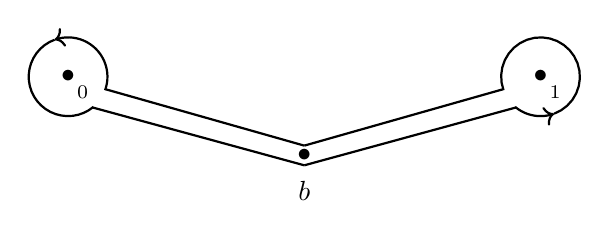
\begin{tikzpicture}
    \node[label=below:{$b$}] at (0,0) {$\bullet$};
    \node[label={[label distance=-3mm]below right:{\scriptsize$1$}}] at (3,1) {$\bullet$};
    \node[label={[label distance=-3mm]below right:{\scriptsize$0$}}] at (-3,1) {$\bullet$};
    \draw[thick,domain=-20:110,->] plot ({0.5*cos(\x)-3}, {0.5*sin(\x)+1});
    \draw[thick,domain=110:310] plot ({0.5*cos(\x)-3}, {0.5*sin(\x)+1});
    \draw[thick,domain=-130:-70,->] plot ({0.5*cos(\x)+3}, {0.5*sin(\x)+1});
    \draw[thick,domain=-70:200] plot ({0.5*cos(\x)+3}, {0.5*sin(\x)+1});
    \draw[thick] (0,0.125) to (-2.52,0.84);
    \draw[thick] (0,0.125) to (2.52,0.84);
    \draw[thick] (0,-0.125) to (-2.69,0.61);
    \draw[thick] (0,-0.125) to (2.69,0.61);
  \end{tikzpicture}
\tag{1}
\]
The purpose of \hyperref[5]{\S5}, \hyperref[7]{\S7}, and \hyperref[15]{\S15} is to construct the language which allows us to do this.
This consists of
\begin{enumerate}[(a)]
  \item giving a motivic sense to $\pi_1(X,x)^{(N)}$, not only to its Lie algebra;
  \item giving a motivic sense to the torsor \hyperref[0.6]{(0.6)} of homotopy classes of paths from $b_1$ to $b_2$;
  \item in \hyperref[figure1]{(1)}, the ``monodromy around $0$'' loop is only unambiguously determined
\oldpage{7~(85)}
    for $b$ ``close to $0$''.
    We must define what it means for a base point to be ``close to $0$''.
\end{enumerate}

Our solution will be to define a motivic linear group as being an Ind-object in the category of motives, endowed with the structure of a commutative Hopf algebra.
To avoid speculation: consider the group in realisation systems, and replace ``motive'' by ``realisation system''.
There is an analogous definition for torsors under a group.
We separately define a notion of ``integer'' structures.
This definition has the advantage that the standard constructions in algebraic geometry (decreasing central series, quotients, pushing forward a $G$-torsor by $G\to H$, twisting by a torsor, \ldots) all translate automatically to the motivic case.
This, in an arbitrary Tannakian category, is explained in \hyperref[5]{\S5}.

In \hyperref[7]{\S7}, we reinterpret these definitions in a language that is closer to that of our applications.
The reader who is displeased by the general nonsense of \hyperref[5]{\S5} and \hyperref[7]{\S7} can take the interpretations given in \hyperref[7]{\S7} as the definition of groups, torsors, \ldots in realisation systems.
Drawback: every standard construction must be redefined in this case.

In the classical definition of $\pi_1$, the role of the base point $b$ can be played by a contractible subset $B$.
It can also be played by a \unsure{filter} $\mathcal{B}$ on $X$ whose base if given by contractible subsets.
For example, if $X$ is a Riemann surface $\overline{X}$ minus a point $s$, and $v$ is a non-zero tangent vector at $s$, with $z$ being a local coordinates centred at $s$, then we can take the contractible subsets
\[
  \begin{gathered}
    0<|z/v|<\varepsilon,
    \quad
    |\arg(z/v)|<\eta:
  \\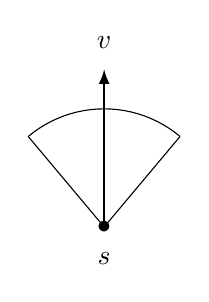
\begin{tikzpicture}
      \node[label={below:{$s$}}] at (0,0) {$\bullet$};
      \draw[thick,-latex] (0,0) to (0,2) node [label={above:{$v$}}] {};
      \draw (0,0) to (50:1.5);
      \draw (0,0) to (130:1.5);
      \draw [domain=50:130] plot ({1.5*cos(\x)}, {1.5*sin(\x)});
    \end{tikzpicture}
  \end{gathered}
\]
The \unsure{filter} $\mathcal{B}(v)$ that they generate is independent of the chosen coordinate.
By this construction, a non-zero tangent vector at $s$ can act as a base point in the definition of $\pi_1$ of $X$.

The same phenomenon occurs in the profinite theory of $\pi_1$, and in the ``de Rham'' theory.
Be aware that $\mathcal{B}(v)=\mathcal{B}(\lambda v)$ for real $\lambda>0$, but that this fact has no analogue in the other theories.
There constructions are explained in \hyperref[15]{\S15}.
They allow us,
\oldpage{8~(86)}
in the definition of the motivic $\pi_1$ of $X$, to take a base point ``at infinity'', like the tangent vector $v$ at $s$.

Let $X=\PP^1\setminus\{0,1,\infty\}$.
An algebraic meaning of ``base point close to $0$'' is ``non-zero tangent vector at $0$''.
For such a base point $b$, the monodromy around $0$ has a motivic meaning: it is a morphism of motivic groups
\[
  \ZZ(1) \to \pi_1(X,b)_\mot.
\]
Here and later on, $\pi_1$ is the pro-unipotent $\pi_1$, defined as the projective limit of the motivic groups $\pi_1(X,b)_\mot^{(N)}$.

We take the base point to be the tangent vector $1$ at $0$.
We have a good reduction $\mod p$ for every $p$, and $\pi_1(X,b)_\mot^{(N)}$ is a linear group in the Tannakian category of motives over $\Spec(\ZZ)$ that are iterated extensions of Tate motives.
\hyperref[8]{\S8} states a conjecture on the $\Ext^1(\QQ,\QQ(k))$ in this category, as well as some consequences.
At the end of \hyperref[16]{\S16}, we make these explicit in the case of $\pi_1(X,b)_\mot^{(N)}$.
I hope that this places the $\zeta(3)$ discovered by Z.~Wojtkoviak in its natural setting.
\hyperref[6]{\S6} is preliminary.
For the essential idea, see \hyperref[6.2]{(6.2)}.

To define the motivic $\pi_1$, we need to patch together the various theories of $\pi_1$ that we have at our disposal, guided by the goal of constructing a motivic group in the sense of \hyperref[5]{\S5}, explained in \hyperref[7]{\S7}.
This is done in \hyperref[10]{\S10} to \hyperref[13]{\S13}, after a reminder (\hyperref[9]{\S9}) on the Mal\v{c}ev theory of nilpotent groups and their Lie algebras.
The result leaves much to be desired.
It is only completely studied for smooth algebraic varieties whose smooth compactifications $\overline{X}$ satisfy $H^1(\overline{X},\scr{O})=0$.
Another complaint: I sometimes only sketch the definition of structures that will be used in future calculations.

In \hyperref[16]{\S16}, we finally explain what the $\ZZ(k)$-torsors from \hyperref[3]{\S3} have to do with the $\pi_1$ of the projective line minus three points.
The justifying calculations are given in \hyperref[19]{\S19}.
We given, in \hyperref[17]{\S17} and \hyperref[18]{\S18}, a geometric explanation of some of their properties.



\section{Terminology and notation}
\label{0}
\oldpage{9~(87)}

\begin{env}{0.1}
\label{0.1}
  We denote inductive limits and projective limits by $\limind$ and $\limproj$.
\end{env}

\begin{env}{0.2}
\label{0.2}
  For a prime number $\ell$, we denote by $\ZZ_\ell$ and $\QQ_\ell$ the completions of $\ZZ$ and $\QQ$ for the $\ell$-adic topology:
  \[
    \begin{aligned}
      \ZZ_\ell &= \limproj \ZZ/\ell^n\ZZ,
    \\\QQ_\ell &= \ZZ_\ell\otimes\QQ.
    \end{aligned}
  \]
  We denote by $\hZZ$ the profinite completion of $\ZZ$, and by $\AA^f$ the ring of finite adeles:
  \[
    \begin{gathered}
      \hZZ \xrightarrow{\sim} \prod_\ell \ZZ_\ell,
    \\\AA^f = \hZZ\otimes\QQ.
    \end{gathered}
  \]
  We denote by $\cQQ$ the algebraic closure of $\QQ$ in $\CC$.
\end{env}

\begin{env}{0.3}
\label{0.3}
  For an abstract group, algebraic group, profinite group, or Lie algebra $A$, we denote by $Z^i(A)$ the descending central series.
  We use the numbering for which $A=Z^1(A)$.
  We denote by $A^{(N)}$ the quotient of $A$ by $Z^{N+1}(A)$.
  In the case of abstract or profinite groups, we denote by $A^{[N]}$ the largest torsion-free quotient of $A^{(N)}$.
\end{env}

\begin{env}{0.4}
\label{0.4}
  We denote by $\otimes$ an extension of scalars.
  For example, if $X$ is a scheme over $k$, and $k'$ is an extension of $k$, then we set
  \[
    X\otimes k'
    \coloneqq X\times_{\Spec(k)}\Spec(k').
  \]
\end{env}

\begin{env}{0.5}
\label{0.5}
  Let $G$ be a sheaf of groups on a site $\cal{S}$, or, equivalently, in a topos $T$.
  Useful particular case: if $\cal{S}$ is a point, then a sheaf is a set and $G$ is a group.
  A \emph{$G$-torsor}, or \emph{torsor under $G$}, is a sheaf $P$ endowed with a right $G$-action such that $P$ is locally isomorphic to $G$ acting on itself by translations on the right.
  We also call such an object a \emph{right $G$-principal homogeneous space}, or a \emph{right principal homogeneous space under $G$}.
\oldpage{10~(88)}
  If $P$ is a $G$-torsor, then a sheaf $X$ on which $G$ acts can be \emph{twisted} by $P$.
  The twisting $X^P$ is the contracted product $P\times^G X=(P\times X)/G$, and is endowed with $\alpha\colon P\to\shIsom(X,X^P)$ satisfying $\alpha(pg)=\alpha(p)g$.

  An \emph{$(H,G)$-bitorsor} (cf. SGA~7, VII.1, or Girard, \emph{Cohomologie non abelienne}, III~1.5) is a space which is simultaneously a left principal homogeneous space under $H$ and a right principal homogeneous space under $G$, with the $G$- and $H$-actions commuting with one another.
  If $P$ is a $G$-torsor, then the sheaf of automorphisms of $P$ is the twisting $G^P$ of $G$ by $P$ (under the action of $G$ on itself by inner automorphisms), and $P$ is a $(G^P,P)$-bitorsor.
  By this construction, the data of an $(H,G)$-bitorsor $P$ is equivalent to the data of a $G$-torsor $P$ along with an isomorphism between $H$ and $G^P$.
  Notation: we will write ${}_HP_G$ to mean that $P$ is an $(H,G)$-bitorsor.

  We will use the following operations on torsors and bitorsors.
  \begin{itemize}
    \item \textbf{Pushing forward:} (or \textbf{transporting}) a $G$-torsor $P$ by $\varphi\colon G\to H$ to obtain an $H$-torsor $\varphi(P)$.
      A \emph{$\varphi$-morphism} from the $G$-torsor $P$ to the $H$-torsor $Q$ is some $u\colon P\to Q$ such that $u(pg)=u(p)\varphi(g)$.
      A $\varphi$-morphism factors uniquely through an isomorphism of $H$-torsors between $\varphi(P)$ and $Q$.
    \item \textbf{Composition:} of a $(G_1,G_2)$-bitorsor $P$ and a $(G_2,G_3)$-bitorsor $Q$:
      the $(G_1,G_3)$-bitorsor $P\circ Q$ given by the contracted product $P\times^{G_2}Q=(P\times Q)/G_2$.
    \item \textbf{Inverse:} of ${}_{G_1}P_{G_2}$:
      the $(G_2,G_1)$-bitorsor $P^{-1}$, unique up to isomorphism, endowed with $(p\mapsto p^{-1})\colon P\to P^{-1}$ such that $(g_1pg_2)^{-1}=g_2^{-1}p^{-1}g_1^{-1}$.

      For $G$-torsors $P$ and $Q$, the sheaf $\shIsom(P,Q)$ of isomorphisms of $G$-torsors from $P$ to $Q$ is the $(G^Q,G^P)$-bitorsor $G\circ P^{-1}$.
  \end{itemize}

  If the site $\cal{S}$ is such that the representable functors $h_S$ are sheaves, then we can transport these operations to $\cal{S}$ via the fully faithful functor $S\mapsto h_S$, with each construction only being defined if it does not leave the collection of representable sheaves.
\end{env}



\section{Mixed motives}
\label{1}
\oldpage{11~(89)}

\begin{env}{1.1}
\label{1.1}
  For algebraic varieties, we have various parallel cohomology theories.
  The most important for us will be de Rham and $\ell$-adic cohomology.

  \begin{itemize}
    \item \textbf{De Rham cohomology.}
      Let $k$ be a field of characteristic~$0$, and $X$ an algebraic variety over $k$.
      Suppose that $X$ is smooth.
      The de Rham cohomology groups $\HH_\DR^i(X)$ are the hypercohomology groups of the de Rham complex:
      \[
        \HH_\DR^i(X)
        \coloneqq \mathbb{H}^i(X,\Omega_{X/k}^\bullet)
      \]
      cf. \cite{G}.
      These are vector spaces over $k$.
      If $k'$ is an extension of $k$, and $X'$ over $k'$ is given by extension of scalars of $X$, then
      \[
        \HH_\DR^i(X') = \HH_\DR^i(X)\otimes_k k'.
      \]
      If $X$ is not smooth, then the de Rham complex no longer gives a reasonable theory.
      We can define the $\HH_\DR^i(X)$ by reduction to the smooth case, by the methods of \cite{D3}, or, if $X$ admits an embedding into a smooth variety $Z$, as the hypercohomology of the de Rham complex of the formal completion of $Z$ along $X$ (R.~Hartshorne, \emph{On the de Rham cohomology of algebraic varieties}, Publ.~Math.~IHES \textbf{45} (1975), p.~5--99);
      more intrinsically, it is the crystalline cohomology of $X$ (A.~Grothendieck, \emph{Crystals and the de Rham cohomology of schemes}, Notes by J.~Coates and O.~Jussila, in: ``dix expos\'{e}s sur la cohomologie des sch\'{e}mas'', North Holland (1968)).
    \item \textbf{$\ell$-adic cohomology.}
      Let $\ell$ be a prime number;
      if $k$ is an algebraically closed field of characteristic~$\neq\ell$, then we have the $\ell$-adic theory $X\mapsto\HH^i(X,\QQ_\ell)$ that associates, to $X$ over $k$, cohomology groups which are vector spaces over $\QQ_\ell$ \cite[\S VI]{SGA5}.
      They are defined from the cohomology groups with coefficients in $\ZZ/(\ell^n)$, and we allow ourselves to give, as reference for a theorem in $\ell$-adic cohomology, the place where its $\ZZ/(\ell^n)$ analogue is proved.
      The $\HH^i(X,\QQ_\ell)$ depend only on $X$.
      In particular, if $k$ is the algebraic closure of $k_0$, and if $X$ is given by extension of scalars of some $X_0$ over $k_0$, then $\Gal(k/k_0)$ acts (semi-$k$-linearly) on $X$, and thus acts on the $\HH^i(X,\QQ_\ell)$.
      This action is continuous.
      If $k'$ is an algebraically closed extension of $k$, and if $X'$ is given by extension of scalars of $X$, then $\HH^i(X,\QQ_\ell)\xrightarrow{\sim}\HH^i(X',\QQ_\ell)$.
      \oldpage{12~(90)}
      This follows by passing to the limit in the base change theorem for a smooth morphism \cite[\S XVI, 1.2]{SGA4}: $k'$ is the filtrant inductive limit of the $k$-algebras $A$ with $\Spec(A)$ smooth over $k$.
  \end{itemize}

  If $k=\CC$, then we have the topological space $X(\CC)$ of points of $X$, as well as its rational cohomology $\HH^\bullet(X(\CC),\QQ)$.
  We have canonical isomorphisms from \cite{G} and (SGA~4, XVI~4.1):
  \[
  \label{1.1.1}
    \HH_\DR^i(X) = \HH^i(X(\CC),\QQ)\otimes_{\QQ}\CC
  \tag{1.1.1}
  \]
  \[
  \label{1.1.2}
    \HH^i(X,\QQ_\ell) = \HH^i(X(\CC),\QQ)\otimes_{\QQ}\QQ_\ell.
  \tag{1.1.2}
  \]

  If $k$ is a field of characteristic~$0$, and $\sigma\colon k\to\CC$ a complex embedding, with $\overline{k}$ the algebraic closure of $k$ in $\CC$ via $\sigma$, then we obtain the isomorphisms
  \[
  \label{1.1.3}
    \HH_\DR^i(X)\otimes_{k,\sigma}\CC = \HH^i(X(\CC),\QQ)\otimes_{\QQ}\CC
  \tag{1.1.3}
  \]
  \[
  \label{1.1.4}
    \HH^i(X\otimes\overline{k},\QQ_\ell) = \HH^i(X(\CC),\QQ)\otimes_{\QQ}\QQ_\ell
  \tag{1.1.4}
  \]
  where $X(\CC)$ is the topological space of points of the complex algebraic variety given by the extension of scalars via $\sigma$ of $X$.
\end{env}


%% Bibliography %%

\nocite{*}

\end{document}
